% answers.tex —— 2011 年·湖北卷·理科 · 参考答案与详细解析片段
% 由 tools/generate_projects.py 依来源总账自 2011/2011_数学真题_湖北理_试题.md + 2011/2011_数学真题_湖北理_解析正文.md + 2011/2011_数学真题_湖北理_答案要点.md 生成，勿手改（改源 MD 后重跑）

\begin{answer}
\gksolhead{1}{}

\textbf{题目}：

$\mathrm i$ 为虚数单位，则 $\left(\dfrac{1+\mathrm i}{1-\mathrm i}\right)^{2011}=$\mbox{（　　）}

（A）$-\mathrm i$

（B）$-1$

（C）$\mathrm i$

（D）$1$

\Needspace{4\baselineskip}
\textbf{解析}
$\dfrac{1+\mathrm i}{1-\mathrm i}=\mathrm i$，故原式 $=\mathrm i^{2011}=\mathrm i^{4\times502+3}=-\mathrm i$。选 A。

\gkanswer{答案：A。}

\end{answer}
\begin{answer}
\gksolhead{2}{}

\textbf{题目}：

已知 $U=\{y\mid y=\log_2x,\ x>1\}$，$P=\left\{y\ \middle|\ y=\dfrac1x,\ x>2\right\}$，则 $\complement_UP=$\mbox{（　　）}

（A）$\left[\dfrac12,+\infty\right)$

（B）$\left(0,\dfrac12\right)$

（C）$(0,+\infty)$

（D）$(-\infty,0)\cup\left[\dfrac12,+\infty\right)$

\Needspace{4\baselineskip}
\textbf{解析}
$x>1$ 时 $y=\log_2x>0$，故 $U=(0,+\infty)$。$x>2$ 时 $0<\dfrac1x<\dfrac12$，故 $P=\left(0,\dfrac12\right)$。于是 $\complement_UP=\left[\dfrac12,+\infty\right)$。选 A。

\gkanswer{答案：A。}

\end{answer}
\begin{answer}
\gksolhead{3}{}

\textbf{题目}：

已知函数 $f(x)=\sqrt3\sin x-\cos x$，$x\in\mathbf R$。若 $f(x)\geqslant1$，则 $x$ 的取值范围为\mbox{（　　）}

（A）$\left\{x\ \middle|\ k\pi+\dfrac\pi3\leqslant x\leqslant k\pi+\pi,\ k\in\mathbf Z\right\}$

（B）$\left\{x\ \middle|\ 2k\pi+\dfrac\pi3\leqslant x\leqslant2k\pi+\pi,\ k\in\mathbf Z\right\}$

（C）$\left\{x\ \middle|\ k\pi+\dfrac\pi6\leqslant x\leqslant k\pi+\dfrac{5\pi}6,\ k\in\mathbf Z\right\}$

（D）$\left\{x\ \middle|\ 2k\pi+\dfrac\pi6\leqslant x\leqslant2k\pi+\dfrac{5\pi}6,\ k\in\mathbf Z\right\}$

\Needspace{4\baselineskip}
\textbf{解析}
\Needspace{5\baselineskip}
$f(x)=2\sin\left(x-\dfrac\pi6\right)\geqslant1\iff\sin\left(x-\dfrac\pi6\right)\geqslant\dfrac12$，故
\nopagebreak[4]
\[2k\pi+\frac\pi6\leqslant x-\frac\pi6\leqslant2k\pi+\frac{5\pi}6,\]
即 $2k\pi+\dfrac\pi3\leqslant x\leqslant2k\pi+\pi$。选 B。

\gkanswer{答案：B。}

\end{answer}
\begin{answer}
\gksolhead{4}{}

\textbf{题目}：

将两个顶点在抛物线 $y^2=2px$（$p>0$）上，另一个顶点是此抛物线焦点的正三角形个数记为 $n$，则\mbox{（　　）}

（A）$n=0$

（B）$n=1$

（C）$n=2$

（D）$n\geqslant3$

\Needspace{4\baselineskip}
\textbf{解析}
设正三角形另两顶点为 $P$、$Q$，焦点 $F\left(\dfrac p2,0\right)$。由对称性，$P$、$Q$ 关于 $x$ 轴对称，$PF=QF$ 且 $PQ=PF$。设 $P(x,y)$，则 $PQ=2|y|$，$PF^2=\left(x-\dfrac p2\right)^2+y^2$。由 $PF=PQ$ 与 $y^2=2px$ 可解出两组对称的解（$y>0$ 与 $y<0$），故 $n=2$。选 C。

\gkanswer{答案：C。}

\end{answer}
\begin{answer}
\gksolhead{5}{}

\textbf{题目}：

已知随机变量 $\xi$ 服从正态分布 $N(2,\sigma^2)$，且 $P(\xi<4)=0.8$，则 $P(0<\xi<2)=$\mbox{（　　）}

（A）$0.6$

（B）$0.4$

（C）$0.3$

（D）$0.2$

\Needspace{4\baselineskip}
\textbf{解析}
\Needspace{5\baselineskip}
正态曲线关于 $x=2$ 对称，$P(\xi>4)=1-0.8=0.2$，故 $P(\xi<0)=0.2$。于是
\nopagebreak[4]
\[P(0<\xi<2)=0.5-P(\xi<0)=0.5-0.2=0.3.\]
选 C。

\gkanswer{答案：C。}

\end{answer}
\begin{answer}
\gksolhead{6}{}

\textbf{题目}：

已知定义在 $\mathbf R$ 上的奇函数 $f(x)$ 和偶函数 $g(x)$ 满足 $f(x)+g(x)=a^x-a^{-x}+2$（$a>0$，且 $a\neq1$）。若 $g(2)=a$，则 $f(2)=$\mbox{（　　）}

（A）$2$

（B）$\dfrac{15}4$

（C）$\dfrac{17}4$

（D）$a^2$

\Needspace{4\baselineskip}
\textbf{解析}
\Needspace{5\baselineskip}
将 $x$ 换成 $-x$：$-f(x)+g(x)=a^{-x}-a^x+2$。与原式相加得 $2g(x)=4$，故 $g(x)=2$。由 $g(2)=a$ 得 $a=2$。于是
\nopagebreak[4]
\[f(2)=2^2-2^{-2}+2-g(2)=4-\frac14+2-2=\frac{15}4.\]
选 B。

\gkanswer{答案：B。}

\end{answer}
\begin{answer}
\gksolhead{7}{}

\textbf{题目}：

如图，用 $K$、$A_1$、$A_2$ 三类不同的元件连接成一个系统。当 $K$ 正常工作且 $A_1$、$A_2$ 至少有一个正常工作时，系统正常工作。已知 $K$、$A_1$、$A_2$ 正常工作的概率依次为 $0.9$、$0.8$、$0.8$，则系统正常工作的概率为\mbox{（　　）}

（A）$0.960$

（B）$0.864$

（C）$0.720$

（D）$0.576$
\nopagebreak[4]
\begin{center}% 2011 年湖北卷理科第 7 题：K 与并联的 A1、A2 组成的系统。
% 来源 PDF：普通高考/2011/2011湖北理.pdf，SHA-256 ba721f03ae90f88887c5cde27ae98dbea165d33c73e5ba45b4e4f56b0638b075。
% 原页：第 1 页第 1 栏上部，书页码 667。
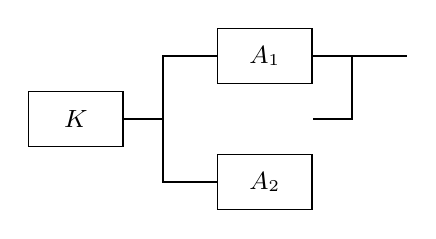
\begin{tikzpicture}[>=stealth, semithick, font=\small]
  \node[draw, minimum width=1.2cm, minimum height=0.7cm] (K) at (0,0) {$K$};
  \node[draw, minimum width=1.2cm, minimum height=0.7cm] (A1) at (2.4,0.8) {$A_1$};
  \node[draw, minimum width=1.2cm, minimum height=0.7cm] (A2) at (2.4,-0.8) {$A_2$};
  \draw (K.east) -- ++(0.5,0) coordinate (x) -- ++(0,0.8) -- (A1.west);
  \draw (x) -- ++(0,-0.8) -- (A2.west);
  \draw (A1.east) -- ++(0.5,0) coordinate (y) -- ++(0,-0.8) -- ++(-0.5,0);
  \draw (y) -- ++(0.7,0);
\end{tikzpicture}
\end{center}
\nopagebreak[4]
\Needspace{4\baselineskip}
\textbf{解析}
\Needspace{5\baselineskip}
$A_1$、$A_2$ 至少一个正常工作的概率为 $1-(1-0.8)^2=0.96$。系统正常工作要求 $K$ 与这一事件同时发生：
\nopagebreak[4]
\[0.9\times0.96=0.864.\]
选 B。

\gkanswer{答案：B。}

\end{answer}
\begin{answer}
\gksolhead{8}{}

\textbf{题目}：

已知向量 $\boldsymbol a=(x+z,3)$，$\boldsymbol b=(2,y-z)$，且 $\boldsymbol a\perp\boldsymbol b$。若 $x$，$y$ 满足不等式 $|x|+|y|\leqslant1$，则 $z$ 的取值范围为\mbox{（　　）}

（A）$[-2,2]$

（B）$[-2,3]$

（C）$[-3,2]$

（D）$[-3,3]$

\Needspace{4\baselineskip}
\textbf{解析}
$\boldsymbol a\perp\boldsymbol b$ 给出 $2(x+z)+3(y-z)=0$，即 $z=2x+3y$。在 $|x|+|y|\leqslant1$ 上，线性函数 $2x+3y$ 的最大值在 $(0,1)$ 取 $3$，最小值在 $(0,-1)$ 取 $-3$，故 $z\in[-3,3]$。选 D。

\gkanswer{答案：D。}

\end{answer}
\begin{answer}
\gksolhead{9}{}

\textbf{题目}：

若实数 $a$，$b$ 满足 $a\geqslant0$，$b\geqslant0$，且 $ab=0$，则称 $a$ 与 $b$ 互补。记 $\varphi(a,b)=\sqrt{a^2+b^2}-a-b$，那么 $\varphi(a,b)=0$ 是 $a$ 与 $b$ 互补的\mbox{（　　）}

（A）必要而不充分条件

（B）充分而不必要条件

（C）充要条件

（D）既不充分也不必要条件

\Needspace{4\baselineskip}
\textbf{解析}
若 $ab=0$（不妨 $b=0$），则 $\varphi=\sqrt{a^2}-a=0$。反之若 $\varphi=0$，则 $\sqrt{a^2+b^2}=a+b$，平方得 $ab=0$。故为充要条件，选 C。

\gkanswer{答案：C。}

\end{answer}
\begin{answer}
\gksolhead{10}{}

\textbf{题目}：

放射性元素由于不断有原子放射出微粒子而变成其他元素，其含量不断减少，这种现象称为衰变。假设在放射性同位素铯 137 的衰变过程中，其含量 $M$（单位：太贝克）与时间 $t$（单位：年）满足函数关系：$M(t)=M_02^{-\frac t{30}}$，其中 $M_0$ 为 $t=0$ 时铯 137 的含量。已知 $t=30$ 时，铯 137 含量的变化率是 $-10\ln2$（太贝克/年），则 $M(60)=$\mbox{（　　）}

（A）$5$ 太贝克

（B）$75\ln2$ 太贝克

（C）$150\ln2$ 太贝克

（D）$150$ 太贝克

\Needspace{4\baselineskip}
\textbf{解析}
\Needspace{5\baselineskip}
$M'(t)=-\dfrac{M_0\ln2}{30}2^{-t/30}$，故
\nopagebreak[4]
\[M'(30)=-\frac{M_0\ln2}{60}=-10\ln2\Longrightarrow M_0=600.\]
于是 $M(60)=600\cdot2^{-2}=150$。选 D。

\gkanswer{答案：D。}

\end{answer}
\begin{answer}
\gksolhead{11}{}

\textbf{题目}：

$\left(x-\dfrac1{3\sqrt x}\right)^{18}$ 的展开式中含 $x^{15}$ 的项的系数为 $\underline{\qquad}$。（结果用数值表示）

\Needspace{4\baselineskip}
\textbf{解析}
\Needspace{5\baselineskip}
通项
\nopagebreak[4]
\[\mathrm C_{18}^k x^{18-k}\left(-\frac1{3\sqrt x}\right)^k=\mathrm C_{18}^k\left(-\frac13\right)^k x^{18-\frac{3k}2}.\]
\Needspace{5\baselineskip}
令 $18-\dfrac{3k}2=15$，得 $k=2$，系数为
\nopagebreak[4]
\[\mathrm C_{18}^2\left(\frac13\right)^2=\frac{153}9=17.\]

\gkanswer{答案：$17$。}

\end{answer}
\begin{answer}
\gksolhead{12}{}

\textbf{题目}：

在 $30$ 瓶饮料中，有 $3$ 瓶已过了保质期。从这 $30$ 瓶饮料中任取 $2$ 瓶，则至少取到 $1$ 瓶已过保质期饮料的概率为 $\underline{\qquad}$。（结果用最简分数表示）

\Needspace{4\baselineskip}
\textbf{解析}
\Needspace{5\baselineskip}
用对立事件：两瓶都未过期有 $\mathrm C_{27}^2$ 种，总数为 $\mathrm C_{30}^2$。故
\nopagebreak[4]
\[P=1-\frac{\mathrm C_{27}^2}{\mathrm C_{30}^2}=1-\frac{351}{435}=\frac{84}{435}=\frac{28}{145}.\]

\gkanswer{答案：$\dfrac{28}{145}$。}

\end{answer}
\begin{answer}
\gksolhead{13}{}

\textbf{题目}：

《九章算术》“竹九节”问题：现有一根 $9$ 节的竹子，自上而下各节的容积成等差数列，上面 $4$ 节的容积共 $3$ 升，下面 $3$ 节的容积共 $4$ 升，则第 $5$ 节的容积为 $\underline{\qquad}$ 升。

\Needspace{4\baselineskip}
\textbf{解析}
\Needspace{5\baselineskip}
设自上而下容积为等差数列 $\{a_n\}$，公差 $d$。则
\nopagebreak[4]
\[a_1+a_2+a_3+a_4=4a_1+6d=3,\qquad a_7+a_8+a_9=3a_1+21d=4.\]
\Needspace{5\baselineskip}
由第一式 $a_1=\dfrac{3-6d}4$，代入第二式：
\nopagebreak[4]
\[\frac{9-18d}4+21d=4\Longrightarrow9+66d=16\Longrightarrow d=\frac7{66}.\]
\Needspace{5\baselineskip}
故
\nopagebreak[4]
\[a_5=a_1+4d=\frac{3-6d}4+4d=\frac34+\frac52\cdot\frac7{66}=\frac34+\frac{35}{132}=\frac{67}{66}.\]

\gkanswer{答案：$\dfrac{67}{66}$。}

\end{answer}
\begin{answer}
\gksolhead{14}{}

\textbf{题目}：

如图，直角坐标系 $xOy$ 所在的平面为 $\alpha$，直角坐标系 $x'Oy'$（其中 $y'$ 轴与 $y$ 轴重合）所在的平面为 $\beta$，$\angle xOx'=45^\circ$。

（1） 已知平面 $\beta$ 内有一点 $P'\left(2\sqrt2,2\right)$，则点 $P'$ 在平面 $\alpha$ 内的射影 $P$ 的坐标为 $\underline{\qquad}$。

（2） 已知平面 $\beta$ 内的曲线 $C'$ 的方程是 $\left(x'-\sqrt2\right)^2+2y'^2-2=0$，则曲线 $C'$ 在平面 $\alpha$ 内的射影 $C$ 的方程是 $\underline{\qquad}$。
\nopagebreak[4]
\begin{center}% 2011 年湖北卷理科第 14 题：平面 α 与 β 成 45°，点与曲线在 α 内的射影。
% 来源 PDF：普通高考/2011/2011湖北理.pdf，SHA-256 ba721f03ae90f88887c5cde27ae98dbea165d33c73e5ba45b4e4f56b0638b075。
% 原页：第 1 页第 2 栏中部，书页码 667。示意。
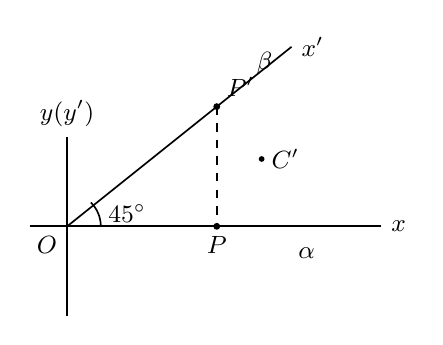
\begin{tikzpicture}[>=stealth, semithick, font=\small, scale=0.95]
  % α 平面（水平）
  \draw (-0.5,0) -- (4.2,0) node[right] {$x$};
  \draw (0,-1.2) -- (0,1.2) node[above] {$y(y')$};
  \node[below left] at (0,0) {$O$};
  \node[below] at (3.2,-0.15) {$\alpha$};
  % β 平面（斜向上 45°）
  \draw (0,0) -- (3.0,2.4) node[right] {$x'$};
  \node[above right] at (2.4,1.9) {$\beta$};
  \draw[dashed] (2.0,1.6) -- (2.0,0) node[below] {$P$};
  \fill (2.0,1.6) circle (1.3pt) node[above right] {$P'$};
  \fill (2.0,0) circle (1.3pt);
  \draw (0.45,0) arc (0:45:0.45) node[midway, right] {$45^\circ$};
  \fill (2.6,0.9) circle (1.1pt) node[right] {$C'$};
\end{tikzpicture}
\end{center}
\nopagebreak[4]
\Needspace{4\baselineskip}
\textbf{解析}
\gksubpart{(1)}
平面 $\beta$ 绕 $y$ 轴旋转 $45^\circ$ 得平面 $\alpha$，点 $(x',y')$ 在 $\alpha$ 内的射影为 $(x'\cos45^\circ,y')$。故 $P'\left(2\sqrt2,2\right)$ 的射影为 $(2,2)$。

\gksubpart{(2)}
\Needspace{5\baselineskip}
将 $x'=\sqrt2x$、$y'=y$ 代入 $C'$：
\nopagebreak[4]
\[\left(\sqrt2x-\sqrt2\right)^2+2y^2-2=0\Longrightarrow2(x-1)^2+2y^2-2=0,\]
即 $(x-1)^2+y^2=1$。

\gkanswer{答案（1）：$(2,2)$。}

\gkanswer{答案（2）：$(x-1)^2+y^2=1$。}

\end{answer}
\begin{answer}
\gksolhead{15}{}

\textbf{题目}：

给 $n$ 个自上而下相连的正方形着黑色或白色。当 $n\leqslant4$ 时，在所有不同的着色方案中，黑色正方形互不相邻的着色方案如图所示。由此推断，当 $n=6$ 时，黑色正方形互不相邻的着色方案共有 $\underline{\qquad}$ 种，至少有两个黑色正方形相邻的着色方案共有 $\underline{\qquad}$ 种。（结果用数值表示）
\nopagebreak[4]
\begin{center}% 2011 年湖北卷理科第 15 题：n=1,2,3,4 时黑色正方形互不相邻的着色方案。
% 来源 PDF：普通高考/2011/2011湖北理.pdf，SHA-256 ba721f03ae90f88887c5cde27ae98dbea165d33c73e5ba45b4e4f56b0638b075。
% 原页：第 1 页第 2 栏下部，书页码 667。黑格用实心表示。
\begin{tikzpicture}[font=\small, scale=0.42]
  \newcommand{\row}[3]{% #1=n, #2=y, #3=pattern string
    \node[left] at (-0.3,#2) {$n=#1$};
    \foreach \c [count=\i from 0] in {#3}{
      \ifnum\c=1
        \fill (\i,#2) rectangle ++(1,1);
      \else
        \draw (\i,#2) rectangle ++(1,1);
      \fi
    }
  }
  \foreach \pat [count=\j from 0] in {0,1}{
    \begin{scope}[xshift=\j*2.0cm]
      \foreach \c [count=\i from 0] in \pat {
        \ifnum\c=1 \fill (\i,0) rectangle ++(1,1); \else \draw (\i,0) rectangle ++(1,1); \fi
      }
    \end{scope}
  }
  \node[left] at (-0.3,0) {$n=1$};
  % n=2
  \begin{scope}[yshift=-2.0cm]
    \foreach \pat [count=\j from 0] in {00,10,01}{
      \begin{scope}[xshift=\j*2.6cm]
        \foreach \c [count=\i from 0] in \pat {
          \ifnum\c=1 \fill (\i,0) rectangle ++(1,1); \else \draw (\i,0) rectangle ++(1,1); \fi
        }
      \end{scope}
    }
    \node[left] at (-0.3,0) {$n=2$};
  \end{scope}
  % n=3
  \begin{scope}[yshift=-4.0cm]
    \foreach \pat [count=\j from 0] in {000,100,010,001,101}{
      \begin{scope}[xshift=\j*3.4cm]
        \foreach \c [count=\i from 0] in \pat {
          \ifnum\c=1 \fill (\i,0) rectangle ++(1,1); \else \draw (\i,0) rectangle ++(1,1); \fi
        }
      \end{scope}
    }
    \node[left] at (-0.3,0) {$n=3$};
  \end{scope}
  % n=4
  \begin{scope}[yshift=-6.0cm]
    \foreach \pat [count=\j from 0] in {0000,1000,0100,0010,0001,1010,1001,0101}{
      \begin{scope}[xshift=\j*4.6cm]
        \foreach \c [count=\i from 0] in \pat {
          \ifnum\c=1 \fill (\i,0) rectangle ++(1,1); \else \draw (\i,0) rectangle ++(1,1); \fi
        }
      \end{scope}
    }
    \node[left] at (-0.3,0) {$n=4$};
  \end{scope}
\end{tikzpicture}
\end{center}
\nopagebreak[4]
\Needspace{4\baselineskip}
\textbf{解析}
设 $n$ 个正方形中黑色互不相邻的方案数为 $F_n$，则 $F_n=F_{n-1}+F_{n-2}$（末格白或末格黑且倒二格白），初值 $F_1=2$、$F_2=3$。算得 $F_3=5$、$F_4=8$、$F_5=13$、$F_6=21$。
全部 $2^6=64$ 种方案中，至少两个黑格相邻的有 $64-21=43$ 种。

\gkanswer{答案：$21$；$43$。}

\end{answer}
\begin{answer}
\gksolhead{16}{}

\textbf{题目}：

设 $\triangle ABC$ 的内角 $A$，$B$，$C$ 所对的边分别为 $a$，$b$，$c$。已知 $a=1$，$b=2$，$\cos C=\dfrac14$。

（1） 求 $\triangle ABC$ 的周长；

（2） 求 $\cos(A-C)$ 的值。

\Needspace{4\baselineskip}
\textbf{解析}
\gksubpart{(1)}
\Needspace{5\baselineskip}
由余弦定理
\nopagebreak[4]
\[c^2=a^2+b^2-2ab\cos C=1+4-2\cdot1\cdot2\cdot\frac14=4,\]
故 $c=2$，周长 $a+b+c=1+2+2=5$。

\gksubpart{(2)}
\Needspace{5\baselineskip}
$\sin C=\sqrt{1-\dfrac1{16}}=\dfrac{\sqrt{15}}4$，且
\nopagebreak[4]
\[\cos A=\frac{b^2+c^2-a^2}{2bc}=\frac{4+4-1}{8}=\frac78,\qquad\sin A=\frac{\sqrt{15}}8.\]
\Needspace{5\baselineskip}
于是
\nopagebreak[4]
\[\cos(A-C)=\cos A\cos C+\sin A\sin C=\frac78\cdot\frac14+\frac{\sqrt{15}}8\cdot\frac{\sqrt{15}}4
=\frac7{32}+\frac{15}{32}=\frac{11}{16}.\]

\gkanswer{答案（1）：$5$。}

\gkanswer{答案（2）：$\dfrac{11}{16}$。}

\end{answer}
\begin{answer}
\gksolhead{17}{}

\textbf{题目}：

提高过江大桥的车辆通行能力可改善整个城市的交通状况。在一般情况下，大桥上的车流速度 $v$（单位：千米/小时）是车流密度 $x$（单位：辆/千米）的函数。当桥上的车流密度达到 $200$ 辆/千米时，造成堵塞，此时车流速度为 $0$；当车流密度不超过 $20$ 辆/千米时，车流速度为 $60$ 千米/小时。研究表明：当 $20\leqslant x\leqslant200$ 时，车流速度 $v$ 是车流密度 $x$ 的一次函数。

（1） 当 $0\leqslant x\leqslant200$ 时，求函数 $v(x)$ 的表达式；

（2） 当车流密度 $x$ 为多大时，车流量（单位时间内通过桥上某观测点的车辆数，单位：辆/小时）$f(x)=x\cdot v(x)$ 可以达到最大，并求出最大值。（精确到 $1$ 辆/小时）

\Needspace{4\baselineskip}
\textbf{解析}
\gksubpart{(1)}
\Needspace{5\baselineskip}
$0\leqslant x\leqslant20$ 时 $v=60$。$20\leqslant x\leqslant200$ 时设 $v=kx+b$，由 $v(20)=60$、$v(200)=0$ 得 $k=-\dfrac13$，$b=\dfrac{200}3$，即 $v=\dfrac{200-x}3$。故
\nopagebreak[4]
\[v(x)=\begin{cases}60,&0\leqslant x\leqslant20,\\[4pt]\dfrac{200-x}3,&20<x\leqslant200.\end{cases}\]

\gksubpart{(2)}
\Needspace{5\baselineskip}
$0\leqslant x\leqslant20$ 时 $f=60x\leqslant1200$。$20\leqslant x\leqslant200$ 时
\nopagebreak[4]
\[f(x)=\frac{x(200-x)}3\leqslant\frac1{3}\left(\frac{200}2\right)^2=\frac{10000}3\approx3333,\]
等号在 $x=100$ 时取到。故 $x=100$ 时车流量最大，约 $3333$ 辆/小时。

\gkanswer{答案（1）：$v(x)=\begin{cases}60,&0\leqslant x\leqslant20,\\[4pt]\dfrac{200-x}3,&20<x\leqslant200.\end{cases}$}

\gkanswer{答案（2）：$x=100$ 时最大，约 $3333$ 辆/小时。}

\end{answer}
\begin{answer}
\gksolhead{18}{}

\textbf{题目}：

如图，已知正三棱柱 $ABC-A_1B_1C_1$ 的各棱长都是 $4$，$E$ 是 $BC$ 的中点，动点 $F$ 在侧棱 $CC_1$ 上，且不与点 $C$ 重合。

（1） 当 $CF=1$ 时，求证：$EF\perp A_1C$；

（2） 设二面角 $C-AF-E$ 的大小为 $\theta$，求 $\tan\theta$ 的最小值。
\nopagebreak[4]
\begin{center}% 2011 年湖北卷理科第 18 题：正三棱柱 ABC-A1B1C1，E 为 BC 中点，F 在 CC1 上。
% 来源 PDF：普通高考/2011/2011湖北理.pdf，SHA-256 ba721f03ae90f88887c5cde27ae98dbea165d33c73e5ba45b4e4f56b0638b075。
% 原页：第 2 页第 1 栏上部，书页码 668。示意。
\begin{tikzpicture}[>=stealth, semithick, font=\small, scale=0.95]
  \coordinate (A) at (0,0);
  \coordinate (B) at (3.0,0);
  \coordinate (C) at (1.5,1.0);
  \coordinate (A1) at (0,3.0);
  \coordinate (B1) at (3.0,3.0);
  \coordinate (C1) at (1.5,4.0);
  \coordinate (E) at ($(B)!0.5!(C)$);
  \coordinate (F) at ($(C)!0.45!(C1)$);
  \draw[thick] (A)--(B)--(C)--cycle;
  \draw[thick] (A1)--(B1)--(C1)--cycle;
  \draw[thick] (A)--(A1) (B)--(B1) (C)--(C1);
  \draw (A1)--(C);
  \draw (E)--(F);
  \draw (A)--(F);
  \draw (A)--(E);
  \fill (E) circle (1.2pt) node[below right] {$E$};
  \fill (F) circle (1.2pt) node[right] {$F$};
  \node[left] at (A) {$A$};
  \node[right] at (B) {$B$};
  \node[below] at (C) {$C$};
  \node[left] at (A1) {$A_1$};
  \node[right] at (B1) {$B_1$};
  \node[above] at (C1) {$C_1$};
\end{tikzpicture}
\end{center}
\nopagebreak[4]
\Needspace{4\baselineskip}
\textbf{解析}
\Needspace{5\baselineskip}
以 $A$ 为原点，$AB$ 为 $x$ 轴，平面 $ABC$ 为 $xy$ 平面建立坐标系。设棱长 $4$：
\nopagebreak[4]
\[A(0,0,0),\ B(4,0,0),\ C(2,2\sqrt3,0),\ A_1(0,0,4),\]
$E$ 为 $BC$ 中点 $E(3,\sqrt3,0)$；设 $F(2,2\sqrt3,h)$（$0<h\leqslant4$）。

\gksubpart{(1)}
\Needspace{5\baselineskip}
$h=1$ 时 $\overrightarrow{EF}=(-1,\sqrt3,1)$，$\overrightarrow{A_1C}=(2,2\sqrt3,-4)$，点积
\nopagebreak[4]
\[-2+6-4=0,\]
故 $EF\perp A_1C$。

\gksubpart{(2)}
\Needspace{5\baselineskip}
平面 $CAF$ 的法向量 $\boldsymbol n_1=\overrightarrow{AC}\times\overrightarrow{AF}=(\sqrt3,-1,0)$；平面 $AEF$ 的法向量
\nopagebreak[4]
\[\boldsymbol n_2=\overrightarrow{AE}\times\overrightarrow{AF}=(\sqrt3h,-3h,4\sqrt3).\]
\Needspace{5\baselineskip}
于是
\nopagebreak[4]
\[\cos\theta=\frac{|\boldsymbol n_1\cdot\boldsymbol n_2|}{|\boldsymbol n_1||\boldsymbol n_2|}
=\frac{3h}{2\sqrt{3h^2+12}},\qquad
\tan^2\theta=\frac{1-\cos^2\theta}{\cos^2\theta}=\frac{h^2+16}{3h^2}.\]
\nopagebreak[4]
\[\tan\theta=\frac{\sqrt{h^2+16}}{\sqrt3h}=\frac1{\sqrt3}\sqrt{1+\frac{16}{h^2}},\]
随 $h$ 增大而减小，故 $h=4$（$F=C_1$）时最小，最小值为 $\dfrac{\sqrt{16+16}}{4\sqrt3}=\dfrac{\sqrt6}3$。

\gkanswer{答案（1）：证明见解析。}

\gkanswer{答案（2）：$\tan\theta$ 的最小值为 $\dfrac{\sqrt6}3$。}

\end{answer}
\begin{answer}
\gksolhead{19}{}

\textbf{题目}：

已知数列 $\{a_n\}$ 的前 $n$ 项和为 $S_n$，且满足 $a_1=a$（$a\neq0$），$a_{n+1}=rS_n$（$n\in\mathbf N^*$，$r\in\mathbf R$，$r\neq-1$）。

（1） 求数列 $\{a_n\}$ 的通项公式；

（2） 若存在 $k\in\mathbf N^*$，使得 $S_{k+1}$，$S_k$，$S_{k+2}$ 成等差数列，试判断：对于任意的 $m\in\mathbf N^*$，且 $m\geqslant2$，$a_{m+1}$，$a_m$，$a_{m+2}$ 是否成等差数列，并证明你的结论。

\Needspace{4\baselineskip}
\textbf{解析}
\gksubpart{(1)}
\Needspace{5\baselineskip}
$n\geqslant2$ 时，$a_{n+1}=rS_n$，$a_n=rS_{n-1}$，相减：
\nopagebreak[4]
\[a_{n+1}-a_n=ra_n\Longrightarrow a_{n+1}=(r+1)a_n.\]
\Needspace{5\baselineskip}
又 $a_2=rS_1=ra$。故
\nopagebreak[4]
\[a_1=a,\qquad a_n=ar(r+1)^{n-2}\ (n\geqslant2).\]

\gksubpart{(2)}
\Needspace{5\baselineskip}
由 $S_{k+1},S_k,S_{k+2}$ 成等差数列：
\nopagebreak[4]
\[2S_k=S_{k+1}+S_{k+2}=2S_k+2a_{k+1}+a_{k+2},\]
\Needspace{5\baselineskip}
故 $a_{k+2}=-2a_{k+1}$，即 $r+1=-2$，$r=-3$。此时对任意 $m\geqslant2$，
\nopagebreak[4]
\[a_{m+1}=-2a_m,\qquad a_{m+2}=4a_m,\]
故 $a_{m+1}+a_{m+2}=2a_m$，即 $a_{m+1},a_m,a_{m+2}$ 成等差数列。

\gkanswer{答案（1）：$a_1=a$，$a_n=ar(r+1)^{n-2}$（$n\geqslant2$）。}

\gkanswer{答案（2）：是；由条件得 $r=-3$，此时 $a_{m+1},a_m,a_{m+2}$ 对任意 $m\geqslant2$ 成等差数列。}

\end{answer}
\begin{answer}
\gksolhead{20}{}

\textbf{题目}：

平面内与两定点 $A_1(-a,0)$，$A_2(a,0)$（$a>0$）连线的斜率之积等于非零常数 $m$ 的点的轨迹，加上 $A_1$，$A_2$ 两点所成的曲线 $C$ 可以是圆、椭圆或双曲线。

（1） 求曲线 $C$ 的方程，并讨论 $C$ 的形状与 $m$ 值的关系；

（2） 当 $m=-1$ 时，对应的曲线为 $C_1$；对给定的 $m\in(-1,0)\cup(0,+\infty)$，对应的曲线为 $C_2$。设 $F_1$，$F_2$ 是 $C_2$ 的两个焦点。试问：在 $C_1$ 上，是否存在点 $N$，使得 $\triangle F_1NF_2$ 的面积 $S=|m|a^2$？若存在，求 $\tan\angle F_1NF_2$ 的值；若不存在，请说明理由。

\Needspace{4\baselineskip}
\textbf{解析}
\gksubpart{(1)}
\Needspace{5\baselineskip}
设动点 $P(x,y)$，$x\neq\pm a$，则
\nopagebreak[4]
\[\frac{y}{x+a}\cdot\frac{y}{x-a}=m\Longrightarrow y^2=m(x^2-a^2),\]
即 $x^2-\dfrac{y^2}{m}=a^2$。
$m>0$ 时为双曲线；$-1<m<0$ 时为焦点在 $x$ 轴的椭圆；$m=-1$ 时为圆 $x^2+y^2=a^2$；$m<-1$ 时为焦点在 $y$ 轴的椭圆。

\gksubpart{(2)}
\Needspace{5\baselineskip}
$m=-1$ 时 $C_1:x^2+y^2=a^2$。对 $m\in(-1,0)\cup(0,+\infty)$，$C_2$ 的半焦距满足
\nopagebreak[4]
\[c^2=a^2(1+m),\qquad F_1F_2=2a\sqrt{1+m}.\]
\Needspace{5\baselineskip}
设 $N(x_0,y_0)$ 在 $C_1$ 上，则 $x_0^2+y_0^2=a^2$，且
\nopagebreak[4]
\[S=\frac12F_1F_2|y_0|=a\sqrt{1+m}\,|y_0|=|m|a^2,\]
\Needspace{5\baselineskip}
故 $|y_0|=\dfrac{|m|a}{\sqrt{1+m}}$。存在条件为 $|y_0|\leqslant a$，即
\nopagebreak[4]
\[\frac{m^2}{1+m}\leqslant1\Longrightarrow m^2-m-1\leqslant0\Longrightarrow\frac{1-\sqrt5}2\leqslant m\leqslant\frac{1+\sqrt5}2.\]
结合 $m\in(-1,0)\cup(0,+\infty)$，存在范围为 $\left[\dfrac{1-\sqrt5}2,0\right)\cup\left(0,\dfrac{1+\sqrt5}2\right]$。

\Needspace{5\baselineskip}
此时 $\cos\angle F_1NF_2=\dfrac{a^2-c^2}{NF_1\cdot NF_2}$，而由面积 $S=\dfrac12NF_1\cdot NF_2\sin\angle F_1NF_2=|m|a^2$ 得 $NF_1\cdot NF_2=\dfrac{2|m|a^2}{\sin\angle F_1NF_2}$。又 $a^2-c^2=-ma^2$，故
\nopagebreak[4]
\[\tan\angle F_1NF_2=\frac{2S}{a^2-c^2}=\frac{2|m|a^2}{-ma^2}.\]
$m<0$ 时为 $2$；$m>0$ 时为 $-2$。

\gkanswer{答案（1）：$C:x^2-\dfrac{y^2}{m}=a^2$（$m\neq0$）；$m>0$ 为双曲线，$-1<m<0$ 为椭圆，$m=-1$ 为圆，$m<-1$ 为椭圆（焦点在 $y$ 轴）。}

\gkanswer{答案（2）：存在条件为 $m\in\left[\dfrac{1-\sqrt5}2,0\right)\cup\left(0,\dfrac{1+\sqrt5}2\right]$；$m<0$ 时 $\tan\angle F_1NF_2=2$，$m>0$ 时 $\tan\angle F_1NF_2=-2$。}

\end{answer}
\begin{answer}
\gksolhead{21}{}

\textbf{题目}：

（1） 已知函数 $f(x)=\ln x-x+1$，$x\in(0,+\infty)$，求函数 $f(x)$ 的最大值；

（2） 设 $a_k$，$b_k$（$k=1,2,\cdots,n$）均为正数，证明：

① 若 $a_1b_1+a_2b_2+\cdots+a_nb_n\leqslant b_1+b_2+\cdots+b_n$，则 $a_1^{b_1}a_2^{b_2}\cdots a_n^{b_n}\leqslant1$；

② 若 $b_1+b_2+\cdots+b_n=1$，则 $\dfrac1n\leqslant b_1^{b_1}b_2^{b_2}\cdots b_n^{b_n}\leqslant b_1^2+b_2^2+\cdots+b_n^2$。

\Needspace{4\baselineskip}
\textbf{解析}
\gksubpart{(1)}
$f'(x)=\dfrac1x-1=\dfrac{1-x}x$，故 $0<x<1$ 时递增、$x>1$ 时递减，最大值 $f(1)=0$。

\gksubpart{(2)}
\Needspace{5\baselineskip}
① 由 $\ln x\leqslant x-1$（$x>0$），
\nopagebreak[4]
\[\ln\left(a_1^{b_1}\cdots a_n^{b_n}\right)=\sum b_i\ln a_i\leqslant\sum b_i(a_i-1)
=\sum a_ib_i-\sum b_i\leqslant0,\]
故 $a_1^{b_1}\cdots a_n^{b_n}\leqslant1$。

\Needspace{5\baselineskip}
② 左边的证明：取 $a_i=\dfrac1{nb_i}$，则 $\sum a_ib_i=1=\sum b_i$，由①得
\nopagebreak[4]
\[\prod\left(\frac1{nb_i}\right)^{b_i}\leqslant1\Longrightarrow\frac1{n\prod b_i^{b_i}}\leqslant1
\Longrightarrow\prod b_i^{b_i}\geqslant\frac1n.\]
\Needspace{5\baselineskip}
右边的证明：令 $A=\sum b_i^2$，取 $a_i=\dfrac{b_i}{A}$，则 $\sum a_ib_i=\dfrac{\sum b_i^2}{A}=1=\sum b_i$，由①得
\nopagebreak[4]
\[\prod\left(\frac{b_i}{A}\right)^{b_i}\leqslant1\Longrightarrow\frac{\prod b_i^{b_i}}{A^{\sum b_i}}\leqslant1
\Longrightarrow\prod b_i^{b_i}\leqslant A=\sum b_i^2.\]

\gkanswer{答案（1）：$0$。}

\gkanswer{答案（2）：证明见解析。}

\end{answer}